\documentclass[UTF8]{ctexart}
\usepackage[colorlinks,linkcolor=blue]{hyperref}
\usepackage[T1]{fontenc}
\usepackage{amsmath}
\usepackage{lmodern}
\usepackage{graphicx} 
\usepackage{float} 
\usepackage{subfigure} 
\usepackage[export]{adjustbox}
\usepackage{tabularx}
\title{Flink 内存模型和管理}
\author{dafeihou@hillstonenet.com}
\date{2022年12月8日}
\begin{document}
    \maketitle
    \section*{说明}
    本文基于Flink版本1.14。

    \newpage
    \section*{内存模型和配置}
    \subsection*{内存模型}
    \paragraph*{}
    参考:\href{https://nightlies.apache.org/flink/flink-docs-release-1.14/docs/deployment/memory/mem_setup/}{Set up Flink’s Process Memory}
    \paragraph*{}
    Flink JVM的内存总量包括Flink自身消耗的内存和运行进程消耗的JVM内存,FLink自身的内存又包括JVM Heap(堆内存)和Off-heap(对外内存)内存。
    \newline 即:

    \begin{minipage}[b]{1.0\linewidth}
        \centering
        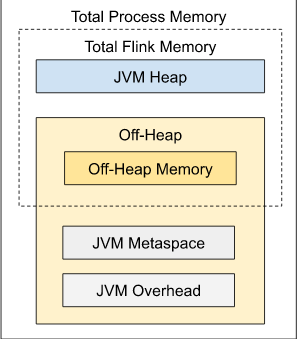
\includegraphics[fbox]{total_memory_model.PNG}
        \label{fig.1}
        \begin{align*}
            TotalFlinkMemory &= JVMHeap\\ &+ OffHeap\\
            TotalProcessMemory &= TotalFlinkMemory\\ &+ JVMMetaspace\\ &+ JVMOverhead
        \end{align*}
    \end{minipage}
    \paragraph*{}
    注:每个组件的作用会在后续说明
    \newpage

    \paragraph*{}
    手动管理Flink内存的方式比较简单,原生提供如下参数可供修改:\\
    \newline
    \begin{minipage}[b]{1\linewidth}
        \centering
        \begin{tabular}{|l|l|l|}
            \hline
            类型&Taskmanager&Jobmanager\\
            \hline
            Total Flink Memory&taskmanager.memory. flink.size&jobmanager.memory.flink.size\\
            \hline
            Total process Memory&taskmanager.memory. process.size&jobmanager.memory.process.size\\
            \hline
        \end{tabular}
    \end{minipage}

    \subsection*{详细的内存参数选项}
    \paragraph*{}
    参考:\href{https://nightlies.apache.org/flink/flink-docs-release-1.14/docs/deployment/config/#memory-configuration}{Memory Configuration}
    \paragraph*{}
    tips:Flink虽然提供了如下参数来修改内存数据,但是官方建议是尽可能不要使用复杂的配置策略,在大多数情况下,用户应该只配置: 
    \begin{itemize}
        \item taskmanager.memory. process.size 调整total process内存
        \item taskmanager.memory. flink.size 调整total flink内存
        \item taskmanager.memory. managed.fraction 根据百分比调整其他内存组件比值
    \end{itemize}
    一些比较详细的配置如下:
    \newline
    \begin{minipage}[b]{1\linewidth}
        \begin{tabular}{|p{3.5cm}|l|l|p{6cm}|}
            \hline
            key&default value&类型&描述\\
            \hline
            jobmanager.memory. enable-jvm-direct-memory-limit & false & boolean & 是否启用jobmanager的直接内存限制\\
            \hline
            jobmanager.memory. flink.size & null & memory & 配置jobmanager的总flink内存大小\\
            \hline
            jobmanager.memory. heap.size & null & memory & 配置jobmanager的堆内存大小,推荐最小值128mb\\
            \hline
            jobmanager.memory. jvm-metaspace.size & 256mb & memory & 配置jobmanager的jvm metaspace大小\\
            \hline
            jobmanager.memory. jvm-overhead.fraction & 0.1 & float & 为jvm overhead保留的total process memory百分比,即预留的一部分堆外内存\\
            \hline
            jobmanager.memory. jvm-overhead.max & 1gb & memory & 保留的最大值\\
            \hline
            jobmanager.memory. jvm-overhead.min & 192mb & memory & 保留的最小值\\
            \hline
            jobmanager.memory. off-heap.size & 128mb & memory & 此参数包含全部的堆外内存分配情况\\
            \hline
            jobmanager.memory. process.size & null & memory & jobmanager的总进程内存大小,即上文total process memory。在容器化部署中,这应该设置为容器内存。\\
            \hline    
        \end{tabular}
    \end{minipage}
    \begin{minipage}[b]{1\linewidth}
        \begin{tabular}{|p{3.5cm}|l|l|p{6cm}|}
            \hline
            key&default value&类型&描述\\
            \hline
            taskmanager.memory. flink.size & null & memory & total flink memory大小\\
            \hline
            taskmanager.memory. framework.heap.size & 128mb & memory & TaskExecutors 的框架堆内存大小,并不分配给slot\\
            \hline
            taskmanager.memory. framework.off-heap.batch-shuffle.size & 32mb & memory & 用于阻塞式shuffle和读取*;需要比taskmanager.memory. framework.off-heap.size小,可以为大规模的批处理加大该配置\\
            \hline
            taskmanager.memory. framework.off-heap.size & 128mb & memory & TaskExecutors 的框架堆外存大小,并不分配给slot\\
            \hline
            taskmanager.memory. jvm-metaspace.size & 256mb & memory & TaskExecutors的JVM metaspace大小\\
            \hline
            taskmanager.memory. jvm-overhead.fraction & 0.1 & float & 为jvm overhead开销保留的堆外内存\\
            \hline
            taskmanager.memory. jvm-overhead.max & 1gb & memory & jvm overhead最大值\\
            \hline
            taskmanager.memory. jvm-overhead.min & 192mb & memory & jvm overhead最小值\\
            \hline
            taskmanager.memory. managed.fraction & 0.4 & float & 如果未明确托管内存大小,则使用total flink memory的百分比做托管内存\\
            \hline
            taskmanager.memory. managed.size & null & memory & TaskExecutors的托管内存大小,用于排序、哈希表、中间结果的缓存、RocksDB的状态后端。\\
            \hline
            taskmanager.memory. network.fraction & 0.1 & float & total flink memory的一部分,用于网络buffer等\\
            \hline
            taskmanager.memory. network.max & 1gb & memory & 最大\\
            \hline
            taskmanager.memory. network.min & 64mb & memory & 最小\\
            \hline
            taskmanager.memory. process.size & null & memory & TaskExecutors的总进程大小,total process memory,容器化部署时应和容器分配的内存一致。\\
            \hline
            taskmanager.memory. task.heap.size & null & memory & TaskExecutors的task heap memory,如果未指定,将是TotalFlinkMemory - 框架堆内存 - 框架堆外内存 - 托管内存 - 托管堆外内存 - 网络内存。\\
            \hline
            taskmanager.memory. task.off-heap.size & 0 bytes & memory & TaskExecutors的task off-heap memory。\\
            \hline    
        \end{tabular}
    \end{minipage}
\end{document}